\documentclass[multi=tikzpicture,border=7pt]{standalone}
\usepackage{ctex,amsmath,bm}
\usepackage{tikz,pgfplots}
\pgfplotsset{compat=1.18}
\usetikzlibrary{arrows.meta,calc,angles,quotes,patterns,positioning,decorations.pathmorphing,3d,intersections}
\tikzset{wire/.style={brown!70!black,very thick},guide/.style={dashed,gray!60},force/.style={->,>=Stealth,thick,red!70!black},velocity/.style={->,>=Stealth,thick,blue!70!black},axis/.style={->,>=Stealth,thick},dim/.style={<->,>=Stealth,thin},body/.style={draw,thick,fill=blue!7},panel/.style={anchor=west,font=\bfseries},hidden/.style={dashed,gray!58,thick},orbit/.style={very thick,blue!70!black}}
\tikzset{charge/.style={circle,draw,fill=blue!12,minimum size=5.5mm,inner sep=0pt},resistor/.style={decorate,decoration={zigzag,segment length=4pt,amplitude=2pt},thick}}
\tikzset{vec/.style={->,>=Stealth,very thick},wall/.style={pattern=north east lines,pattern color=gray},nodept/.style={circle,fill=white,draw,inner sep=1.5pt}}
\begin{document}
% 1 question-01
\begin{tikzpicture}[x=1cm,y=1cm,font=\small]
\begin{scope}[shift={(-3,0)}]\draw[thick](-2,0)--(2.5,0);\draw[fill=blue!8](0,1)circle(1);\fill(0,1)circle(1.5pt)node[above]{$C$};\draw[velocity](0,1)--(.65,1)node[above]{$v_0$};\draw[thick](.866,.5)--(2.3,.5);\draw[thick](.866,.5)--(2.3,0);\draw[dim](2.5,0)--(2.5,.5)node[right]{$h=r/2$};\end{scope}
\begin{scope}[shift={(3,0)}]\draw[thick](-2,0)--(2.5,0);\draw[fill=orange!8](0,1)circle(1);\fill(0,1)circle(1.5pt)node[below]{$C$};\draw[velocity](0,1)--(.65,1)node[above]{$v_0$};\draw[thick](.866,1.5)--(2.3,1.5);\draw[thick](.866,1.5)--(2.3,0);\draw[dim](2.5,0)--(2.5,1.5)node[right]{$h=3r/2$};\end{scope}\node at(0,-.8){均先接触突出棱角；高棱角下方留空};
\end{tikzpicture}

% 2 solution-01
\begin{tikzpicture}[x=1cm,y=1cm,font=\small]
\begin{scope}[shift={(-3,0)}]\draw[fill=blue!8](0,0)circle(1);\fill(.866,-.5)circle(2pt)node[right]{$A_1$};\draw[force](.866,-.5)--(-.173,.1)node[above]{$\boldsymbol n_1$};\draw[velocity](0,0)--(-.6,1.039)node[above]{$\boldsymbol v_1$};\draw[guide](0,0)--(1.3,0);\draw[dim](0,0)--(.866,-.5)node[midway,below]{$r$};\node at(0,-1.8){低棱角：向左上反射};\end{scope}
\begin{scope}[shift={(3,0)}]\draw[fill=orange!8](0,1)circle(1);\draw[thick](-1.7,0)--(1.7,0);\fill(.866,1.5)circle(2pt)node[above]{$A_2$};\draw[velocity](0,1)--(-.6,-.039)node[left]{$\boldsymbol v^-$};\draw[force](0,0)--(.9,0)node[right]{$J_x>0$};\draw[force](0,0)--(0,.8)node[right]{$J_y$};\draw[->](.3,.8)arc(-30:-300:.35)node[right]{$\omega^-<0$};\node at(0,-.8){球底滑速$v_x^-+r\omega^-<0$};\end{scope}
\end{tikzpicture}

% 3 question-02
\begin{tikzpicture}[x=1cm,y=1cm,font=\small]
\begin{scope}[shift={(-3,0)}]\draw[fill=blue!10](0,0)circle(1.3);\draw[fill=white](0,0)circle(.65);\draw[dim](0,0)--(1.3,0)node[midway,below]{$R$};\draw[dim](0,0)--(0,.65)node[left]{$R/2$};\node at(0,-1.9){均匀体电荷，总量$Q$};\end{scope}\draw[velocity](-.9,0)--(.9,0)node[midway,above]{$\lambda=3/2$};
\begin{scope}[shift={(3,0)}]\draw[fill=orange!10](0,0)circle(1.95);\draw[fill=white](0,0)circle(.975);\draw[dim](0,0)--(1.95,0)node[midway,below]{$3R/2$};\draw[dim](0,0)--(0,.975)node[left]{$3R/4$};\node at(0,-2.5){膨胀后：仍均匀，总量$Q$};\end{scope}
\end{tikzpicture}

% 4 solution-02
\begin{tikzpicture}[x=1cm,y=1cm,font=\small]
\begin{scope}[shift={(0,0)}]\draw[axis](-1.8,0)--(5.2,0)node[right]{$s/R$};\draw[thick](0,0)circle(0.75);\fill[blue](0.125,0)circle(2pt)node[above]{$q$};\fill[orange](4.5,0)circle(2pt)node[below]{$q^\prime=-6q$};\node at(1.8,2){空腔内解：$a=3R/4$};\node[below]at(0.125,-.4){$s=0.125R$};\node[above]at(4.5,.4){$s^\prime=4.5R$};\end{scope}\begin{scope}[shift={(0,-4)}]\draw[axis](-1.8,0)--(5.2,0)node[right]{$s/R$};\draw[thick](0,0)circle(1.5);\fill[blue](3,0)circle(2pt)node[above]{$q$};\fill[orange](0.75,0)circle(2pt)node[below]{$q^\prime=-q/2$};\node at(1.8,2){外域解：$b=3R/2$};\node[below]at(3,-.4){$s=3R$};\node[above]at(0.75,.4){$s^\prime=0.75R$};\end{scope}\node at(1.8,-6){中性补偿$Q_0=3q/2$在外表面；内域只加常量势$kq/R$};
\end{tikzpicture}

% 5 question-03
\begin{tikzpicture}[x=1cm,y=1cm,font=\small]
\draw[axis](0,0)--(3,0)node[right]{$y$};\draw[axis](0,0)--(0,3.8)node[above]{$z$};\draw[axis](0,0)--(-1,-.8)node[below]{$x$};
\draw[body](0,0)--(.7,3.2)--(2.6,2.4)--cycle;\draw[fill=blue!8](1.65,2.8)ellipse(.98 and .25);\draw[velocity](0,0)--(2.1,3.57)node[above]{$\omega$};\fill(1.2375,2.1)circle(2pt)node[right]{$C$};\node at(.25,-.3){$O$};\draw[->](0,.9)arc(90:60:.9)node[midway,above]{$\theta$};\node at(2.8,1.5){$H$，全顶角$\beta$};\draw[->](-.4,1.4)arc(180:40:.6 and .2)node[right]{$\Omega$};
\end{tikzpicture}

% 6 solution-03
\begin{tikzpicture}[x=1cm,y=1cm,font=\small]
\draw[axis](0,0)--(3.5,0)node[right]{$y$};\draw[axis](0,0)--(0,3.8)node[above]{$z$};\draw[axis](0,0)--(-1.6,-1.2)node[left]{$x$};\draw[velocity](0,0)--(2.1,3.2)node[right]{$\boldsymbol L\simeq I_3\omega_3\boldsymbol e_3$};\fill(1.575,2.4)circle(2pt)node[right]{$C$};\draw[guide](1.575,0)--(1.575,2.4);\draw[force](1.575,2.4)--(1.575,1.2)node[right]{$Mg$};\draw[force](0,0)--(-1.2,0)node[left]{$F_y$};\draw[force](0,0)--(0,1.3)node[left]{$F_z$};\draw[force](0,0)--(.9,.675)node[right]{$\tau_g$沿$-x$};\node at(1,-1.8){$F_z=Mg,\quad F_y=-M\Omega^2(3H/4)\sin\theta$};
\end{tikzpicture}

% 7 question-04
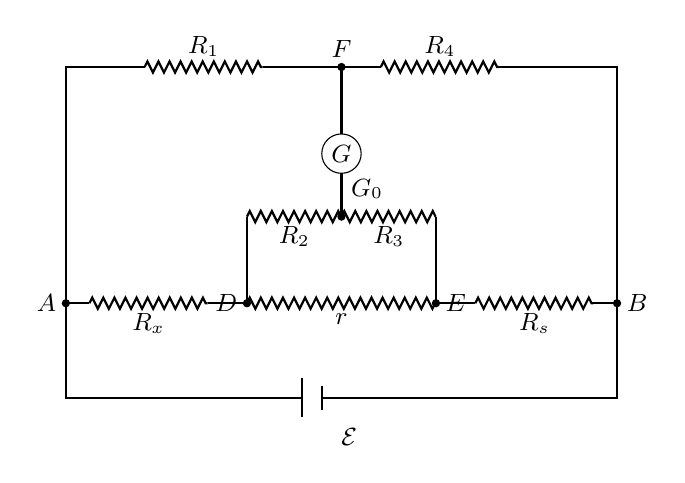
\begin{tikzpicture}[x=1cm,y=1cm,font=\small]
\draw[thick](0,0)--(0,3)--(1,3);\draw[resistor](1,3)--(2.5,3)node[midway,above]{$R_1$};\draw[thick](2.5,3)--(4,3);\draw[resistor](4,3)--(5.5,3)node[midway,above]{$R_4$};\draw[thick](5.5,3)--(7,3)--(7,0);
\draw[resistor](.3,0)--(1.8,0)node[midway,below]{$R_x$};\draw[thick](0,0)--(.3,0);\draw[thick](1.8,0)--(2.3,0);\draw[resistor](2.3,0)--(4.7,0)node[midway,below]{$r$};\draw[thick](4.7,0)--(5.2,0);\draw[resistor](5.2,0)--(6.7,0)node[midway,below]{$R_s$};\draw[thick](6.7,0)--(7,0);
\draw[thick](2.3,0)--(2.3,1.1);\draw[resistor](2.3,1.1)--(3.5,1.1)node[midway,below]{$R_2$};\draw[resistor](3.5,1.1)--(4.7,1.1)node[midway,below]{$R_3$};\draw[thick](4.7,1.1)--(4.7,0);
\draw[thick](3.5,1.1)--(3.5,1.65);\draw(3.5,1.9)circle(.25)node{$G$};\draw[thick](3.5,2.15)--(3.5,3);\fill(3.5,3)circle(1.5pt)node[above]{$F$};\fill(3.5,1.1)circle(1.5pt)node[above right,yshift=1mm]{$G_0$};\fill(2.3,0)circle(1.5pt)node[left]{$D$};\fill(4.7,0)circle(1.5pt)node[right]{$E$};\fill(0,0)circle(1.5pt)node[left]{$A$};\fill(7,0)circle(1.5pt)node[right]{$B$};\draw[thick](0,0)--(0,-1.2)--(3,-1.2);\draw[thick](3,-1.45)--(3,-.95);\draw[thick](3.25,-1.35)--(3.25,-1.05);\draw[thick](3.25,-1.2)--(7,-1.2)--(7,0);\node at(3.6,-1.7){$\mathcal E$};
\end{tikzpicture}

% 8 solution-04
\begin{tikzpicture}[x=1cm,y=1cm,font=\small]
\begin{scope}[shift={(-4,0)}]\fill(0.0,0)circle(2pt)node[below]{$\bar r_2$};\fill(0.6,0)circle(2pt)node[below]{$\bar r_3$};\fill(1.2,0)circle(2pt)node[below]{$\bar r_4$};\fill(1.7999999999999998,0)circle(2pt)node[below]{$\bar r_5$};\fill(2.4,0)circle(2pt)node[below]{$\bar r_6$};\fill(3.0,0)circle(2pt)node[below]{$\bar r_7$};\fill(3.5999999999999996,0)circle(2pt)node[below]{$\bar r_8$};\fill(4.2,0)circle(2pt)node[below]{$\bar r_9$};\draw[->,red!70](0.0,.25)to[bend left=28](2.4,.25);\draw[->,red!70](0.6,.25)to[bend left=28](3.0,.25);\draw[->,red!70](1.2,.25)to[bend left=28](3.5999999999999996,.25);\draw[->,red!70](1.7999999999999998,.25)to[bend left=28](4.2,.25);\node at(2,1.6){每条跨4个砝码};\node at(2,-1.1){四差相加再除以16};\end{scope}\begin{scope}[shift={(3,0)}]\draw[wall](-.4,2.8)rectangle(.4,3);\draw[body](-.25,0)rectangle(.25,2.8);\draw[force](0,0)--(0,-.8)node[below]{$mg$};\draw[dim](-.8,0)--(-.8,2.8)node[midway,left]{$L$};\draw[force](.35,1.5)--(1.3,1.5)node[right]{$\varepsilon_r=-\mu\varepsilon_l$};\node at(.8,-1.4){$\Delta R/R=(1+2\mu)\varepsilon_l$};\end{scope}
\end{tikzpicture}

% 9 question-05
\begin{tikzpicture}[x=1cm,y=1cm,font=\small]
\begin{scope}[shift={(-3,0)}]\draw[body](-2,-.5)--(1,-.5)--(2,1.3)--(-1,1.3)--cycle;\draw[thick](-2,-.5)--(-2,-.7)--(1,-.7)--(1,-.5);\draw[fill=orange!20](-.6,.5)ellipse(.16 and .3);\draw[fill=orange!20](.7,.5)ellipse(.16 and .3);\node[above]at(-.6,.8){$P_1$};\node[above]at(.7,.8){$P_2$};\draw[dim](-.6,1.3)--(.7,1.3)node[midway,above]{$l$};\node at(0,-1.4){二维：厚度$d$，柱半径$a$};\end{scope}\begin{scope}[shift={(3,0)}]\draw[fill=blue!10](-1,0)circle(.35);\draw[fill=orange!10](1,0)circle(.35);\draw[force](-1,0)--(-1.7,.8)node[left]{$P_1$};\draw[force](1,0)--(1.7,.8)node[right]{$P_2$};\draw[dim](-1,-.8)--(1,-.8)node[midway,below]{$l\gg a$};\node at(0,1.6){三维：远处$T_0$};\node at(0,-1.7){$P_i>0$表示装置给球供热};\end{scope}
\end{tikzpicture}

% 10 solution-05
\begin{tikzpicture}[x=1cm,y=1cm,font=\small]
\begin{scope}[shift={(-3,0)}]\foreach\r in{.4,.8,1.2}{\draw[blue!25](0,0)circle(\r);}\draw[force](0,0)--(1.3,.6)node[right]{$P$};\node at(0,-1.8){$A=2\pi rd$};\node at(0,-2.5){$T(r)-T(a)=-\frac{P}{2\pi\sigma d}\ln\frac ra$};\end{scope}\begin{scope}[shift={(3,0)}]\draw[fill=blue!8](-1,0)circle(.4);\draw[fill=orange!8](1,0)circle(.4);\draw[velocity](-.6,0)--(.6,0)node[midway,above]{交叉温升};\node at(0,1.5){球面热流：$A=4\pi r^2$};\node at(0,-1.3){$4\pi\sigma\Delta_1=P_1/a+P_2/l$};\node at(0,-2.1){$4\pi\sigma\Delta_2=P_1/l+P_2/a$};\end{scope}
\end{tikzpicture}

% 11 question-06
\begin{tikzpicture}[x=1cm,y=1cm,font=\small]
\draw[axis](-2.6,0)--(2.7,0)node[right]{原卷轴线};\draw[thick](-.3,0)circle(1.8);\draw[thick](.2,0)circle(1.15);\fill(-.3,0)circle(2pt)node[below]{$O_1$};\fill(.2,0)circle(2pt)node[above]{$O_2$};\draw[dim](-.3,-2.3)--(.2,-2.3)node[midway,below]{$d$};\node at(-1.3,1.3){$R$};\node at(.9,.6){$r$};\node at(0,2.7){原卷内含圆：须先核验所用成像模型};
\end{tikzpicture}

% 12 solution-06
\begin{tikzpicture}[x=1cm,y=1cm,font=\small]
\draw[axis](-4,0)--(4.4,0)node[right]{$X$};\draw[very thick](0,-1.5)--(0,1.8)node[above]{透镜$O$};\draw[blue!80](-2.414213562373095,0)circle(1);\draw[orange!80!black](2.414213562373095,0)circle(1);\fill(-1,0)circle(2pt)node[below]{$F$};\fill(1,0)circle(2pt)node[below]{$F'$};\fill(-2.414213562373095,0)circle(2pt)node[below]{$O_1$};\fill(2.414213562373095,0)circle(2pt)node[below]{$O_2$};\draw[force](-1.00000,0.00000)--(-1.70711,0.70711)node[midway,above]{$p=f$};\draw[gray!65](-3.08049,0.74571)--(0.00000,0.00000)--(1.48066,-0.35843);\draw[blue!60](-3.08049,0.74571)--(0.00000,0.74571)--(1.48066,-0.35843);\node at(0,-2.1){$f=R=r=1,\ D=-1-\sqrt2$};\node at(0,-2.8){物、像圆等半径；前后焦点分别在$X=\mp f$};
\end{tikzpicture}

% 13 question-07
\begin{tikzpicture}[x=1cm,y=1cm,font=\small]
\begin{scope}[shift={(-4,0)}]\draw[wall](-.3,-.8)rectangle(0,1);\draw[body](0,0)rectangle(3.5,.3);\draw[fill=blue!25](.5,.3)rectangle(1,.45)node[above]{$R_2,R_3$};\draw[fill=orange!25](.5,-.15)rectangle(1,0)node[below]{$R_1,R_4$};\draw[force](3.5,.15)--(3.5,-1)node[below]{$mg$};\draw[dim](0,1)--(3.5,1)node[midway,above]{$l$};\draw[dim](0,-.8)--(.75,-.8)node[midway,below]{$x$};\end{scope}
\begin{scope}[shift={(2,0)}]\draw[thick](0,-1)--(0,1.5)--(.4,1.5);\draw[resistor](.4,1.5)--(1.4,1.5)node[midway,above]{$R_2$};\draw[thick](1.4,1.5)--(2,1.5);\draw[resistor](2,1.5)--(3,1.5)node[midway,above]{$R_1$};\draw[thick](3,1.5)--(3.4,1.5)--(3.4,-1);\draw[thick](0,-1)--(.4,-1);\draw[resistor](.4,-1)--(1.4,-1)node[midway,below]{$R_4$};\draw[thick](1.4,-1)--(2,-1);\draw[resistor](2,-1)--(3,-1)node[midway,below]{$R_3$};\draw[thick](3,-1)--(3.4,-1);\draw[thick](1.7,1.5)--(1.7,.5);\draw(1.7,.25)circle(.25)node{$V$};\draw[thick](1.7,0)--(1.7,-1);\fill(1.7,1.5)circle(1.5pt)node[above]{$A$};\fill(1.7,-1)circle(1.5pt)node[below]{$B$};\node at(-.25,.25){$+$};\node at(3.65,.25){$-$};\node at(1.7,-2){电源跨左右端，读数$U_A-U_B$};\end{scope}
\end{tikzpicture}

% 14 solution-07
\begin{tikzpicture}[x=1cm,y=1cm,font=\small]
\draw[wall](-.3,-.8)rectangle(0,.8);\draw[orbit](0.00000,-0.00000)--(0.05063,-0.00025)--(0.10127,-0.00098)--(0.15190,-0.00219)--(0.20253,-0.00387)--(0.25316,-0.00602)--(0.30380,-0.00864)--(0.35443,-0.01170)--(0.40506,-0.01522)--(0.45570,-0.01918)--(0.50633,-0.02357)--(0.55696,-0.02840)--(0.60759,-0.03365)--(0.65823,-0.03931)--(0.70886,-0.04539)--(0.75949,-0.05187)--(0.81013,-0.05875)--(0.86076,-0.06603)--(0.91139,-0.07368)--(0.96203,-0.08172)--(1.01266,-0.09014)--(1.06329,-0.09892)--(1.11392,-0.10806)--(1.16456,-0.11756)--(1.21519,-0.12741)--(1.26582,-0.13760)--(1.31646,-0.14812)--(1.36709,-0.15898)--(1.41772,-0.17016)--(1.46835,-0.18166)--(1.51899,-0.19346)--(1.56962,-0.20558)--(1.62025,-0.21799)--(1.67089,-0.23070)--(1.72152,-0.24369)--(1.77215,-0.25697)--(1.82278,-0.27051)--(1.87342,-0.28433)--(1.92405,-0.29841)--(1.97468,-0.31274)--(2.02532,-0.32732)--(2.07595,-0.34215)--(2.12658,-0.35721)--(2.17722,-0.37250)--(2.22785,-0.38802)--(2.27848,-0.40375)--(2.32911,-0.41970)--(2.37975,-0.43585)--(2.43038,-0.45220)--(2.48101,-0.46875)--(2.53165,-0.48548)--(2.58228,-0.50239)--(2.63291,-0.51948)--(2.68354,-0.53673)--(2.73418,-0.55415)--(2.78481,-0.57172)--(2.83544,-0.58945)--(2.88608,-0.60731)--(2.93671,-0.62531)--(2.98734,-0.64345)--(3.03797,-0.66171)--(3.08861,-0.68008)--(3.13924,-0.69857)--(3.18987,-0.71716)--(3.24051,-0.73586)--(3.29114,-0.75465)--(3.34177,-0.77352)--(3.39241,-0.79248)--(3.44304,-0.81151)--(3.49367,-0.83061)--(3.54430,-0.84977)--(3.59494,-0.86899)--(3.64557,-0.88825)--(3.69620,-0.90757)--(3.74684,-0.92691)--(3.79747,-0.94629)--(3.84810,-0.96570)--(3.89873,-0.98512)--(3.94937,-1.00456)--(4.00000,-1.02400);\draw[thick](0.00000,-0.25000)--(0.05063,-0.25025)--(0.10127,-0.25098)--(0.15190,-0.25219)--(0.20253,-0.25387)--(0.25316,-0.25602)--(0.30380,-0.25864)--(0.35443,-0.26170)--(0.40506,-0.26522)--(0.45570,-0.26918)--(0.50633,-0.27357)--(0.55696,-0.27840)--(0.60759,-0.28365)--(0.65823,-0.28931)--(0.70886,-0.29539)--(0.75949,-0.30187)--(0.81013,-0.30875)--(0.86076,-0.31603)--(0.91139,-0.32368)--(0.96203,-0.33172)--(1.01266,-0.34014)--(1.06329,-0.34892)--(1.11392,-0.35806)--(1.16456,-0.36756)--(1.21519,-0.37741)--(1.26582,-0.38760)--(1.31646,-0.39812)--(1.36709,-0.40898)--(1.41772,-0.42016)--(1.46835,-0.43166)--(1.51899,-0.44346)--(1.56962,-0.45558)--(1.62025,-0.46799)--(1.67089,-0.48070)--(1.72152,-0.49369)--(1.77215,-0.50697)--(1.82278,-0.52051)--(1.87342,-0.53433)--(1.92405,-0.54841)--(1.97468,-0.56274)--(2.02532,-0.57732)--(2.07595,-0.59215)--(2.12658,-0.60721)--(2.17722,-0.62250)--(2.22785,-0.63802)--(2.27848,-0.65375)--(2.32911,-0.66970)--(2.37975,-0.68585)--(2.43038,-0.70220)--(2.48101,-0.71875)--(2.53165,-0.73548)--(2.58228,-0.75239)--(2.63291,-0.76948)--(2.68354,-0.78673)--(2.73418,-0.80415)--(2.78481,-0.82172)--(2.83544,-0.83945)--(2.88608,-0.85731)--(2.93671,-0.87531)--(2.98734,-0.89345)--(3.03797,-0.91171)--(3.08861,-0.93008)--(3.13924,-0.94857)--(3.18987,-0.96716)--(3.24051,-0.98586)--(3.29114,-1.00465)--(3.34177,-1.02352)--(3.39241,-1.04248)--(3.44304,-1.06151)--(3.49367,-1.08061)--(3.54430,-1.09977)--(3.59494,-1.11899)--(3.64557,-1.13825)--(3.69620,-1.15757)--(3.74684,-1.17691)--(3.79747,-1.19629)--(3.84810,-1.21570)--(3.89873,-1.23512)--(3.94937,-1.25456)--(4.00000,-1.27400);\draw[force](4,-1.024)--(4,-2)node[below]{$mg$};\node at(1.7,1.25){上表面受拉，$R_2,R_3$增加};\node at(1.5,-3.5){下表面受压，$R_1,R_4$减小};\node[anchor=west]at(5,.2){$M(x)=mg(l-x)$};\node[anchor=west]at(5,-1){$\varepsilon=6mg(l-x)/(E_Ybt^2)$};\node[anchor=west]at(5,-2.2){$|\Delta U|=K\mathcal E|\varepsilon|$};
\end{tikzpicture}

% 15 question-08
\begin{tikzpicture}[x=1cm,y=1cm,font=\small]
\draw[axis](-2,0)--(2.8,0)node[right]{东};\draw[axis](0,-2)--(0,2.4)node[above]{北};\draw[fill=blue!20](-1.5,0)circle(.18)node[above]{$3m$};\draw[velocity](-1.3,0)--(-.35,0)node[midway,below]{$0.8c$};\draw[fill=orange!20](0,-1.5)circle(.18)node[right]{$2m$};\draw[velocity](0,-1.3)--(0,-.35)node[midway,right]{$0.6c$};\draw[force](0,0)--(1.4,.525)node[above]{$\boldsymbol P$};\node at(0,-2.7){无辐射：末态质量$4m$与$m$};
\end{tikzpicture}

% 16 solution-08
\begin{tikzpicture}[x=1cm,y=1cm,font=\small]
\draw[axis](-.5,0)--(5.7,0)node[right]{东};\draw[axis](0,-1.8)--(0,4.6)node[above]{北};\draw[orbit](4.58357,1.71884)--(4.56178,1.77319)--(4.53754,1.82653)--(4.51088,1.87879)--(4.48184,1.92990)--(4.45046,1.97979)--(4.41679,2.02839)--(4.38087,2.07564)--(4.34274,2.12145)--(4.30248,2.16579)--(4.26012,2.20857)--(4.21572,2.24975)--(4.16936,2.28927)--(4.12109,2.32706)--(4.07098,2.36309)--(4.01910,2.39729)--(3.96551,2.42963)--(3.91031,2.46006)--(3.85355,2.48853)--(3.79532,2.51501)--(3.73571,2.53946)--(3.67478,2.56184)--(3.61263,2.58213)--(3.54935,2.60030)--(3.48501,2.61631)--(3.41971,2.63016)--(3.35355,2.64182)--(3.28660,2.65127)--(3.21896,2.65851)--(3.15073,2.66351)--(3.08201,2.66628)--(3.01287,2.66681)--(2.94343,2.66511)--(2.87378,2.66116)--(2.80401,2.65498)--(2.73422,2.64658)--(2.66450,2.63596)--(2.59496,2.62315)--(2.52569,2.60816)--(2.45678,2.59101)--(2.38833,2.57172)--(2.32044,2.55033)--(2.25319,2.52685)--(2.18669,2.50133)--(2.12102,2.47380)--(2.05627,2.44430)--(1.99254,2.41286)--(1.92990,2.37953)--(1.86846,2.34436)--(1.80829,2.30740)--(1.74947,2.26869)--(1.69209,2.22829)--(1.63623,2.18626)--(1.58196,2.14266)--(1.52937,2.09753)--(1.47851,2.05096)--(1.42946,2.00299)--(1.38230,1.95371)--(1.33708,1.90317)--(1.29386,1.85144)--(1.25272,1.79860)--(1.21369,1.74472)--(1.17685,1.68988)--(1.14223,1.63414)--(1.10989,1.57759)--(1.07988,1.52031)--(1.05222,1.46237)--(1.02697,1.40386)--(1.00415,1.34485)--(0.98380,1.28543)--(0.96594,1.22568)--(0.95061,1.16568)--(0.93782,1.10552)--(0.92758,1.04527)--(0.91992,0.98502)--(0.91484,0.92486)--(0.91236,0.86487)--(0.91247,0.80512)--(0.91517,0.74571)--(0.92046,0.68672)--(0.92834,0.62822)--(0.93879,0.57030)--(0.95179,0.51303)--(0.96734,0.45650)--(0.98540,0.40079)--(1.00596,0.34597)--(1.02898,0.29212)--(1.05444,0.23931)--(1.08229,0.18761)--(1.11251,0.13710)--(1.14504,0.08785)--(1.17984,0.03992)--(1.21687,-0.00662)--(1.25607,-0.05171)--(1.29739,-0.09527)--(1.34078,-0.13726)--(1.38616,-0.17761)--(1.43349,-0.21628)--(1.48269,-0.25319)--(1.53369,-0.28832)--(1.58643,-0.32159)--(1.64084,-0.35298)--(1.69683,-0.38244)--(1.75433,-0.40992)--(1.81326,-0.43538)--(1.87354,-0.45880)--(1.93509,-0.48014)--(1.99782,-0.49938)--(2.06164,-0.51647)--(2.12647,-0.53141)--(2.19221,-0.54416)--(2.25878,-0.55472)--(2.32609,-0.56306)--(2.39403,-0.56918)--(2.46252,-0.57307)--(2.53146,-0.57472)--(2.60076,-0.57413)--(2.67032,-0.57131)--(2.74005,-0.56624)--(2.80984,-0.55895)--(2.87960,-0.54944)--(2.94924,-0.53772)--(3.01866,-0.52382)--(3.08776,-0.50775)--(3.15645,-0.48952)--(3.22464,-0.46918)--(3.29222,-0.44674)--(3.35910,-0.42224)--(3.42520,-0.39571)--(3.49042,-0.36719)--(3.55468,-0.33671)--(3.61787,-0.30432)--(3.67992,-0.27007)--(3.74074,-0.23400)--(3.80024,-0.19615)--(3.85835,-0.15660)--(3.91498,-0.11537)--(3.97005,-0.07255)--(4.02350,-0.02818)--(4.07523,0.01768)--(4.12519,0.06496)--(4.17331,0.11359)--(4.21951,0.16352)--(4.26373,0.21466)--(4.30592,0.26695)--(4.34601,0.32032)--(4.38395,0.37469)--(4.41969,0.42999)--(4.45317,0.48614)--(4.48435,0.54307)--(4.51320,0.60069)--(4.53966,0.65892)--(4.56370,0.71769)--(4.58528,0.77692)--(4.60439,0.83651)--(4.62099,0.89640)--(4.63505,0.95649)--(4.64657,1.01671)--(4.65552,1.07696)--(4.66189,1.13718)--(4.66567,1.19727)--(4.66686,1.25715)--(4.66545,1.31673)--(4.66145,1.37595)--(4.65487,1.43471)--(4.64571,1.49293)--(4.63398,1.55053)--(4.61970,1.60743)--(4.60289,1.66356)--(4.58357,1.71884);\draw[orange!85!black,thick](0.00000,0.00000)--(4.85012,-1.21503)node[right]{$-14.1^\circ$};\draw[orange!85!black,thick](0.00000,0.00000)--(2.85528,4.10456)node[right]{$55.2^\circ$};\draw[force](0,0)--(2.78947,1.04605)node[below right]{$C,\ \theta_C=20.6^\circ$};\node at(3,-2.4){蓝椭圆：$4m$粒子末态动量端点；橙线为切线};
\end{tikzpicture}

\end{document}
